% !TEX root = master_thesis.tex
\chapter{Extraction of the beam asymmetries $\Sigma_{\eta}$ and $\Sigma_{\eta'}$}
The beam asymmetry $\Sigma$ is observable when a linearly polarized photon beam and unpolarized liquid hydrogen target are employed. The polarized cross section $\frac{\text{d}\sigma}{\text{d}\Omega}_\text{pol}$ is not symmetric in the azimuthal angle $\phi$ anymore as opposed to the unpolarized cross section $\frac{\text{d}\sigma}{\text{d}\Omega}_0$. It is rather modulated by a cosine dependence which scales with the polarization observable $\Sigma$ and the (linear) beam polarization $p_\gamma$, see equation \eqref{eq:asym} \cite{san}.
\begin{equation}
	\frac{\text{d}\sigma}{\text{d}\Omega}_\text{pol}=\frac{\text{d}\sigma}{\text{d}\Omega}_0\cdot\left[1-p_\gamma\Sigma\cos\left(2\varphi\right)\right]
	\label{eq:asym}
\end{equation}
Since the incident photon beam is polarized, photon momentum $\vec{k}$ and polarization $\vec{\epsilon}$ span a plane which is referred to as the beam polarization plane. This plane is tilted by the angle $\varphi$ with respect to the reaction plane which is defined by the final state momenta. Naturally, this plane builds the angle $\phi$ in the laboratory system. At the same time the angle of the beam polarization plane in the same reference frame is defined as $\alpha$. It holds 
\begin{equation}
	\varphi=\alpha-\phi.
\end{equation} Figure \ref{fig:angles} illustrates definitions of all angles and planes. 
 \begin{figure}[htbp]
	\centering
	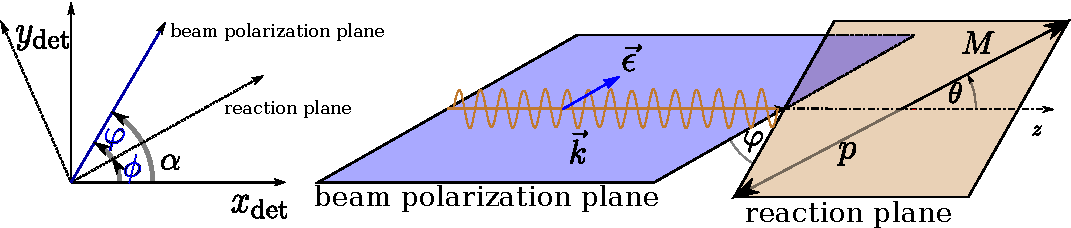
\includegraphics[width=\linewidth]{../DPG2022/figs/angles.pdf}
	\caption{Left: Definition of angles $\alpha,\phi,\varphi$. Right: Photon momentum $\vec{k}$ and polarization  $\vec{\epsilon}$ define the beam polarization plane while the reaction plane is defined by the recoil proton $p$ and produced meson $M$.}
	\label{fig:angles}
\end{figure} 
Theoretically the beam asymmetry can be determined by a measurement of the cross section and a fit using equation \eqref{eq:asym}. However, when calculating polarized cross sections, it is important to have good control over flux normalization and detector acceptance in three dimensions $(E_\gamma,\cos\theta,\phi)$. To avoid this, the measurement of asymmetries can be used to access the polarization observable $\Sigma$ instead. Particularly, data is taken for two distinct orthogonal polarization settings corresponding to $\alpha=\pm\SI{45}{\degree}$.

This chapter will illustrate the process of determining the beam asymmetry for $\eta$ and $\eta'$ photoproduction. The published results of $\Sigma_{\eta}$ \cite{farahphd,eta} are used to check the accuracy and functionality of employed bayesian methods. Bayesian methods, as well as traditional frequentist approaches are used afterwards to extract new results for $\Sigma_{\eta'}$. First, the used methods will be presented and subsequently their application for each final state, respectively.
\section{Methods}
methods
\subsection{Event yield asymmetries}
\subsubsection{Frequentist}
\subsubsection{Bayesian}
\subsection{Event based fit}
\subsubsection{Frequentist}
\subsubsection{Bayesian}
\section{Determination of $\Sigma_{\eta}$ using Bayesian statistics}
\subsection{Event yield asymmetries}
\subsubsection{Application of method to toy Monte Carlo data}
\subsubsection{Application of method to data}
\subsection{Event based fit}
\subsubsection{Application of method to toy Monte Carlo data}
\subsubsection{Application of method to data}
\section{Determination of $\Sigma_{\eta'}$}
\subsection{Application of event based fit to toy Monte Carlo data}
\subsection{Application of event based fit to data}